\section{Results}
\subsection{Results of single models}
Before merging the three models together it must be controlled whether each model is implemented correctly for itself. The figures of the models simulation results are the guide for this. Sometimes there are discrepancies between the published model and the figure which should represents the model.  Hereafter, the implementation process for each of the models is described.\\
To better retrace the implementation steps it is recommended to read the paper for the hog \cite{Zi_2010}, ion \cite{Gerber_2016} and volume model  \cite{volumeModel}.

\subsubsection{Ion model}
The challenges with the implementation of the ion model were, that the presented equations, initial values and parameters did not result in the intended system behavior. \\
After an in-depth analysis of the equation there were two anomalies:

\begin{enumerate}
	\item the calculation of the change of the inner proton ion concentration has \emph{Bf} as an undefined parameter
	\item the fluxes have the wrong units
\end{enumerate}

For solving the problem with the undefined parameter the ODE was constructed by deriving the formula for the calculation of the pH value for diluted solution equation \ref{pHforDilution}
\begin{equation*}
	pH = - log_{10}([H^+])\\
\end{equation*}
\begin{equation}\label{pHforDilution}
	\frac{d}{dt}pH = \frac{d}{dt}(-log_{10}([H^+])) = - \frac{1}{ln(10)} \frac{d}{dt}ln([H^+]) = - \frac{1}{ln(10)}\frac{1}{H^+} \frac{dH^+}{dt}
\end{equation}
and combine it with the equation \ref{pHchange} for the change of the pH Value as a result of proton flux (\cite{martinafroehlich})
\begin{equation}\label{pHchange}
	\frac{d}{dt}pH_{in} = \frac{J_H \cdot Surface}{V_{in} \cdot pbc}
\end{equation}
	
The equation \ref{usedProtonFlux} 
\begin{equation}\label{usedProtonFlux}
- \frac{1}{ln(10)} \frac{1}{H^+}\frac{dH^+}{dt} = \frac{J_H \cdot Surface}{V_{in} \cdot pbc}\\
\Rightarrow \frac{dH^+}{dt}=-\frac{J_H \cdot Surface \cdot ln(10) \cdot H^+}{V_{in} \cdot pbc}
\end{equation}

was used for modeling the change of the inner proton concentration. $pbc$ is the proton buffer capacity.\\\\
To solve the problem with the wrong units it was identified, that the equation for the reported fluxes only missed the unit Kelvin ($K$) in its numerator. Multiplying the equation with the temperature $T$ solved this problem and resulted in the equation \ref{IonFlux}.
This model represents the model with the initial values and global quantities and volumes from Table 4 in the ion paper \cite{Gerber_2016}. The phenomenological and stoichiometric coefficients were adopted from the original Copasi ion model file. In figure 2 the implemented ion model is visualized.
\begin{figure}[htbp]
	
	\begin{minipage}{0,5\textwidth}
		
		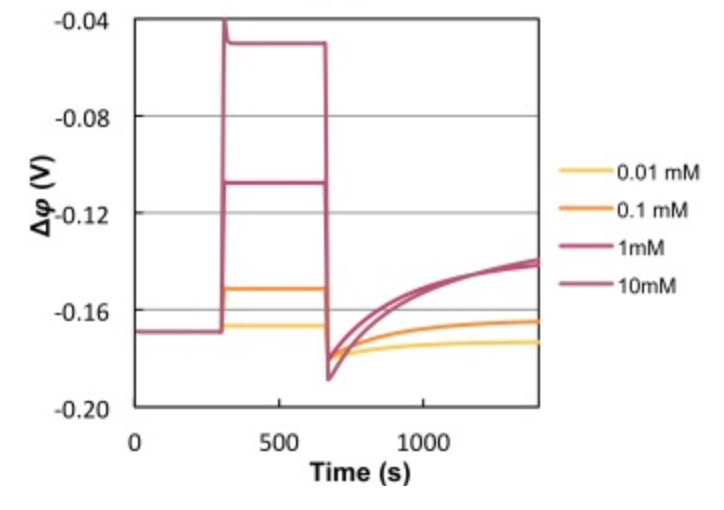
\includegraphics[width=\textwidth]{picture/Ion_Paper.png}
		
		\label{IonPaper} 
	\end{minipage}
	\begin{minipage}{0,5\textwidth}
		
		\includegraphics[width=\textwidth]{picture/ion_examine.png}
		
		\label{IonImplemented} 
	\end{minipage}
	\caption{left: membrane voltage in the ion paper for different NaCl stimulus (0.01 mM - 10 mM) at time $t=300s$ and glucose at $t=600s$; right: the simulated implemented ion model for the same stimulus range }
\end{figure}

\subsubsection{Hog model}
For the implementation of the hog model, the \textit{Table S1-S3} and the Matlab code for the used NaCl impulse in \textit{Code S1 } in the supporting informations of the paper were implemented in the python3 environment. No difficulties were encountered. The only problems occur with the handling of the intended stimulus time length. See figure 3 for the validation of the implemented model.\newpage

\begin{figure}[h!]
	
	\begin{minipage}{0,5\textwidth}
		
		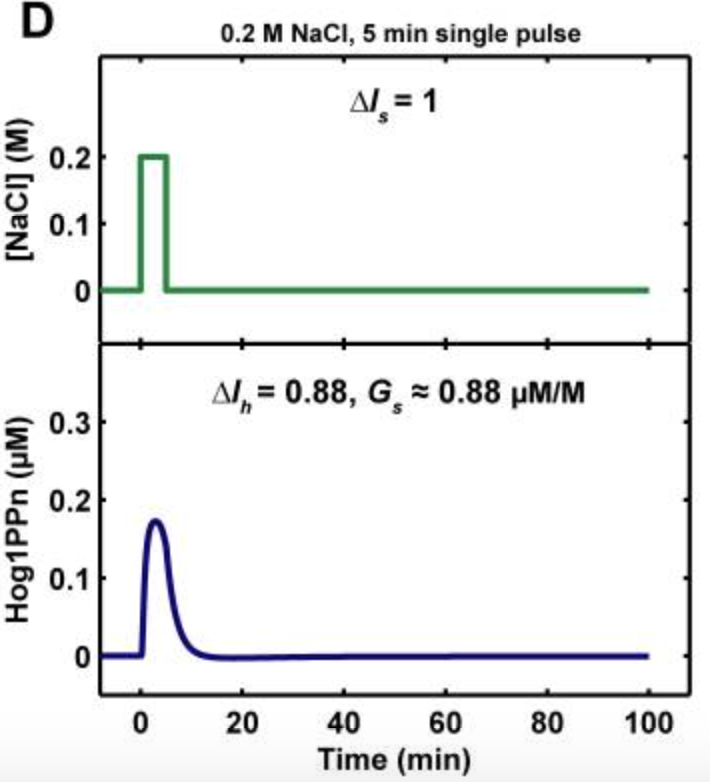
\includegraphics[width=\textwidth]{picture/Hog_Paper.png}
		
		\label{hogPaper} 
	\end{minipage}
	\begin{minipage}{0,5\textwidth}
		
		\includegraphics[width=\textwidth]{picture/hog_examine.png}
		
		
	\end{minipage}
	\label{hogImplemented} 
	\caption{Hog1PPn expression after a 0.2 M NaCl single pulse stimulus for $t=0-300s$; left: hog model from the paper; right: the simulated implemented hog model}
\end{figure}

\subsubsection{Volume model}
The volume model could not be implemented with only the corresponding paper because the model wants to describes the change of the non-osmolytic volume $V_b$ but missed to note down an equation for this.\\
After consultation with my supervisor and one of the author of the model about this information gap, it was recommended that I use the already implemented volume model in their local network "YCM" as a template. After translating this template in my own software structure, no problems were encountered. In the appendix I documented the used ODE, algebraic equation, parameter and initial values for this model, visualized in figure 4. \newpage
\begin{figure}[htbp]
	
	\begin{minipage}{0,5\textwidth}
		
		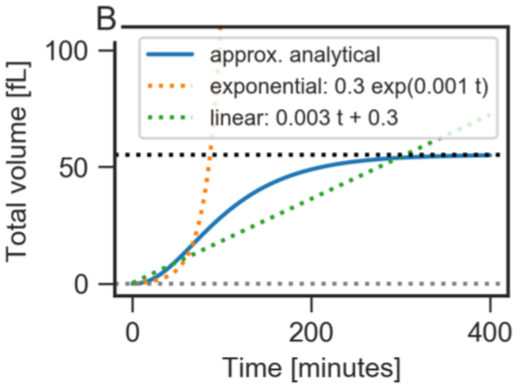
\includegraphics[width=\textwidth]{picture/Volume_Paper.png}
		
		\label{volumePaper} 
	\end{minipage}
	\begin{minipage}{0,5\textwidth}
		
		\includegraphics[width=\textwidth]{picture/volume_examine.png}
		
		\label{volumeImplemented} 
	\end{minipage}
	\caption{no stimulus; left: volume model from the paper; right: the simulated implemented volume model}
\end{figure}


\subsection{Merging of the models}
The process of merging models is a tricky task. There exists some good guideline \cite{Liebermeister2008ValidityAC} for this.
Hereafter, the used essential steps are sketched:
\begin{enumerate}
	\item equations: One of the first steps in the process of model merging is to control whether there is a conflict between assumptions of the description of the biological systems. Conflicts must be resolved by combining equation terms or discard some informations
	\item names: Find all the overlaps in the variable and parameter naming and convert them to a common set of names
	\item units: Standardize all used units for the parameter and initial values to a common set. In this process new factors where give to individual values if the unit changes requires that.
\end{enumerate}
Changes in the equation design (ODE and algebraic equation) were done in the process of merging the models and are presented below in table \ref{changesOnTheModels}:\newpage

\begin{table} [h]
	\footnotesize
\begin{center} 
	\caption{changes in the equation design}
\begin{tabular} {p{3.5cm} l p{6cm} }
%&  \multicolumn{2}{c}{changing equation}  \\ \hline
\toprule
& changes & reason\\
\midrule
internal / external osmolyte concentration & $c = \sum ([Ionen]+[$other osmolyte$])$ & simplification\\ 
\addlinespace[9pt]
internal / external pressure & $\pi = c \cdot R \cdot T	$ & simplification\\
\addlinespace[9pt]
ion x changes & $\frac{J_x \cdot CellSurface}{CellVolume} \cdot 10^{6}$ & unit harmonization without changing flux $J_x$ calculation\\
\addlinespace[9pt]
sorbitol stimulus & $\frac{d}{dt}[Sorbitol]=0$ & implementation of sorbitol stimulus with the assumption that sorbitol can not diffuse over the plasma membrane; in ODE format because this generates less memory data\\
\addlinespace[9pt]
uptake / dilution of osmotic active compounds & removed & replaced with the equations for ion and glycerol\\
\bottomrule
\end{tabular}
\label{changesOnTheModels}
\end{center}
\end{table}
The NaCl stimulus approach from the hog model was not adopted. The response to a stimulus takes place with stopping the ODE solver and adding the stimulus concentration to the last values of the affected substances.\\
In the whole process of merging we must consider their biochemical interpretation to maintain the plausibility of the model \cite{Liebermeister2008ValidityAC}. No parameter value was changed in its biological interpretation.\\\\
Initial values were changed because, as we can see in figure \ref{IntersectionsOfTheModels}

\begin{figure}[h!]
	\begin{center}
		\begin{minipage}{0,8\textwidth}
			
			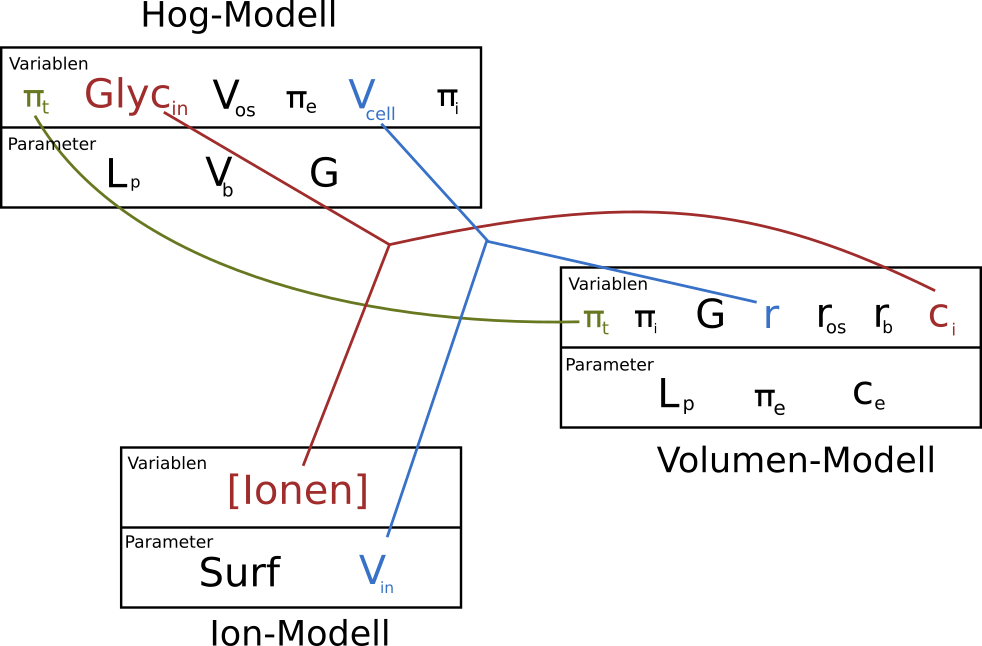
\includegraphics[width=\textwidth]{picture/model_intersections.png}
			\caption{intersections between the three single models parameter and variables; colored: significant different assumptions for same intended behavior} 
			\label{IntersectionsOfTheModels} 
		\end{minipage}
	\end{center}
\end{figure}

 multiple components are used in several models. These components have different quantities in the initial assumptions. One of the main difference was the assumption of the cell volume $V_{cell}$ in the hog model ($V_{cell}=58fL $) and the volume model ($V_{cell} \approx 0.27fL$). To solve this problem we simulated the volume model until $V_{cell}$ also has the value of $58fL$. We assumed the ODE values at this time point as the initial values for the corresponding substance in the merged model. \\\\
We removed the volume related variables and $\pi_t$ from the hog model because the calculation of $\pi_t$ in the volume model was based on updated insights.


% bis hier hin alles gut. Bleibt so. Gleichungen aber noch anschauen.
\subsection{Combined model}
In figure \ref{Interplay} the interplay between the key components in the combined model in response to a hyperosmotic extracellular shock are visualized.
\begin{figure}[h!]
	\begin{center}
		\begin{minipage}{0,75\textwidth}
			
			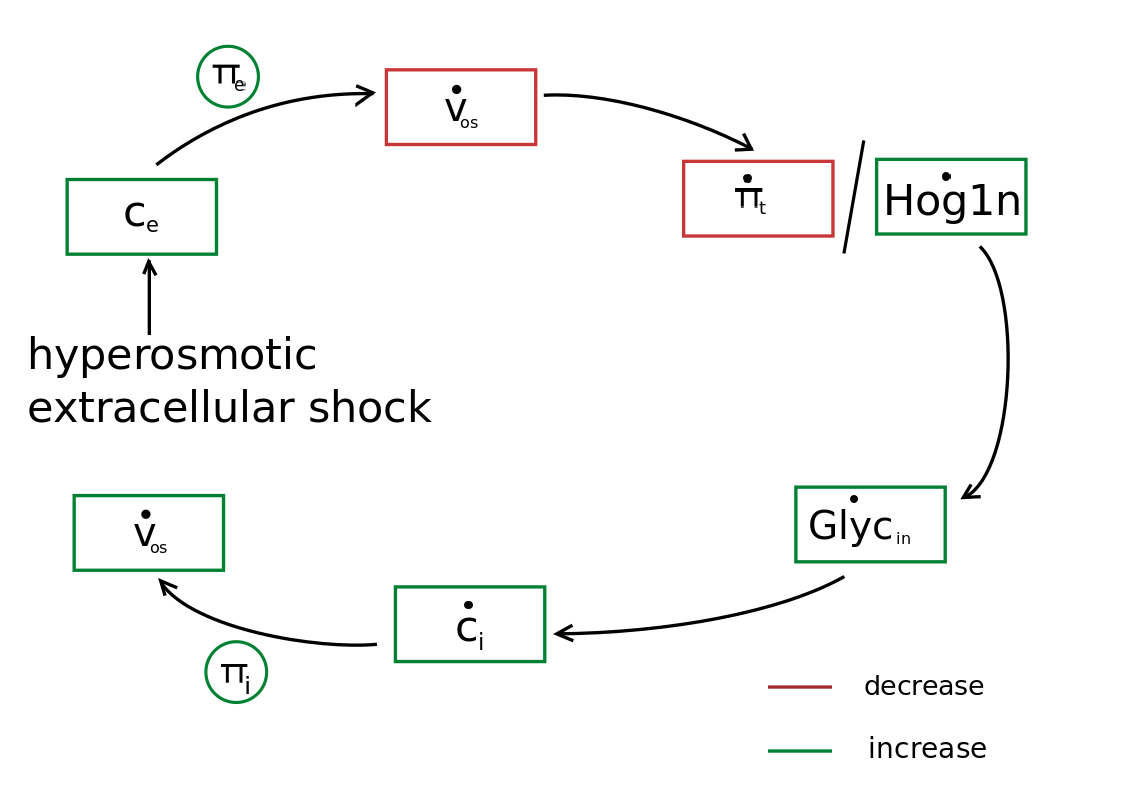
\includegraphics[width=\textwidth]{picture/Interplay.png}
			\caption{interplay between the key components in the combined model} 
			\label{Interplay} 
		\end{minipage}
	\end{center}
\end{figure}
For the analysis and validation of the merged model we choose the nuclear phosphorylated Hog1 (Hog1PPn) as the control substance. Hog1PPn is also used in the hog model as the output because it regulates the expression of hundred of genes \cite{Zi_2010}. We borrowed the idea of a dose response curve with a calculation of the area under the curve (AUC) of Hog1PPn from the theme field pharmacokinetic as a visualized output, showed below in figure \ref{DrugResponseCurve}.  \newpage
\begin{figure}[h!]
	\begin{center}
		\begin{minipage}{0,70\textwidth}
			
			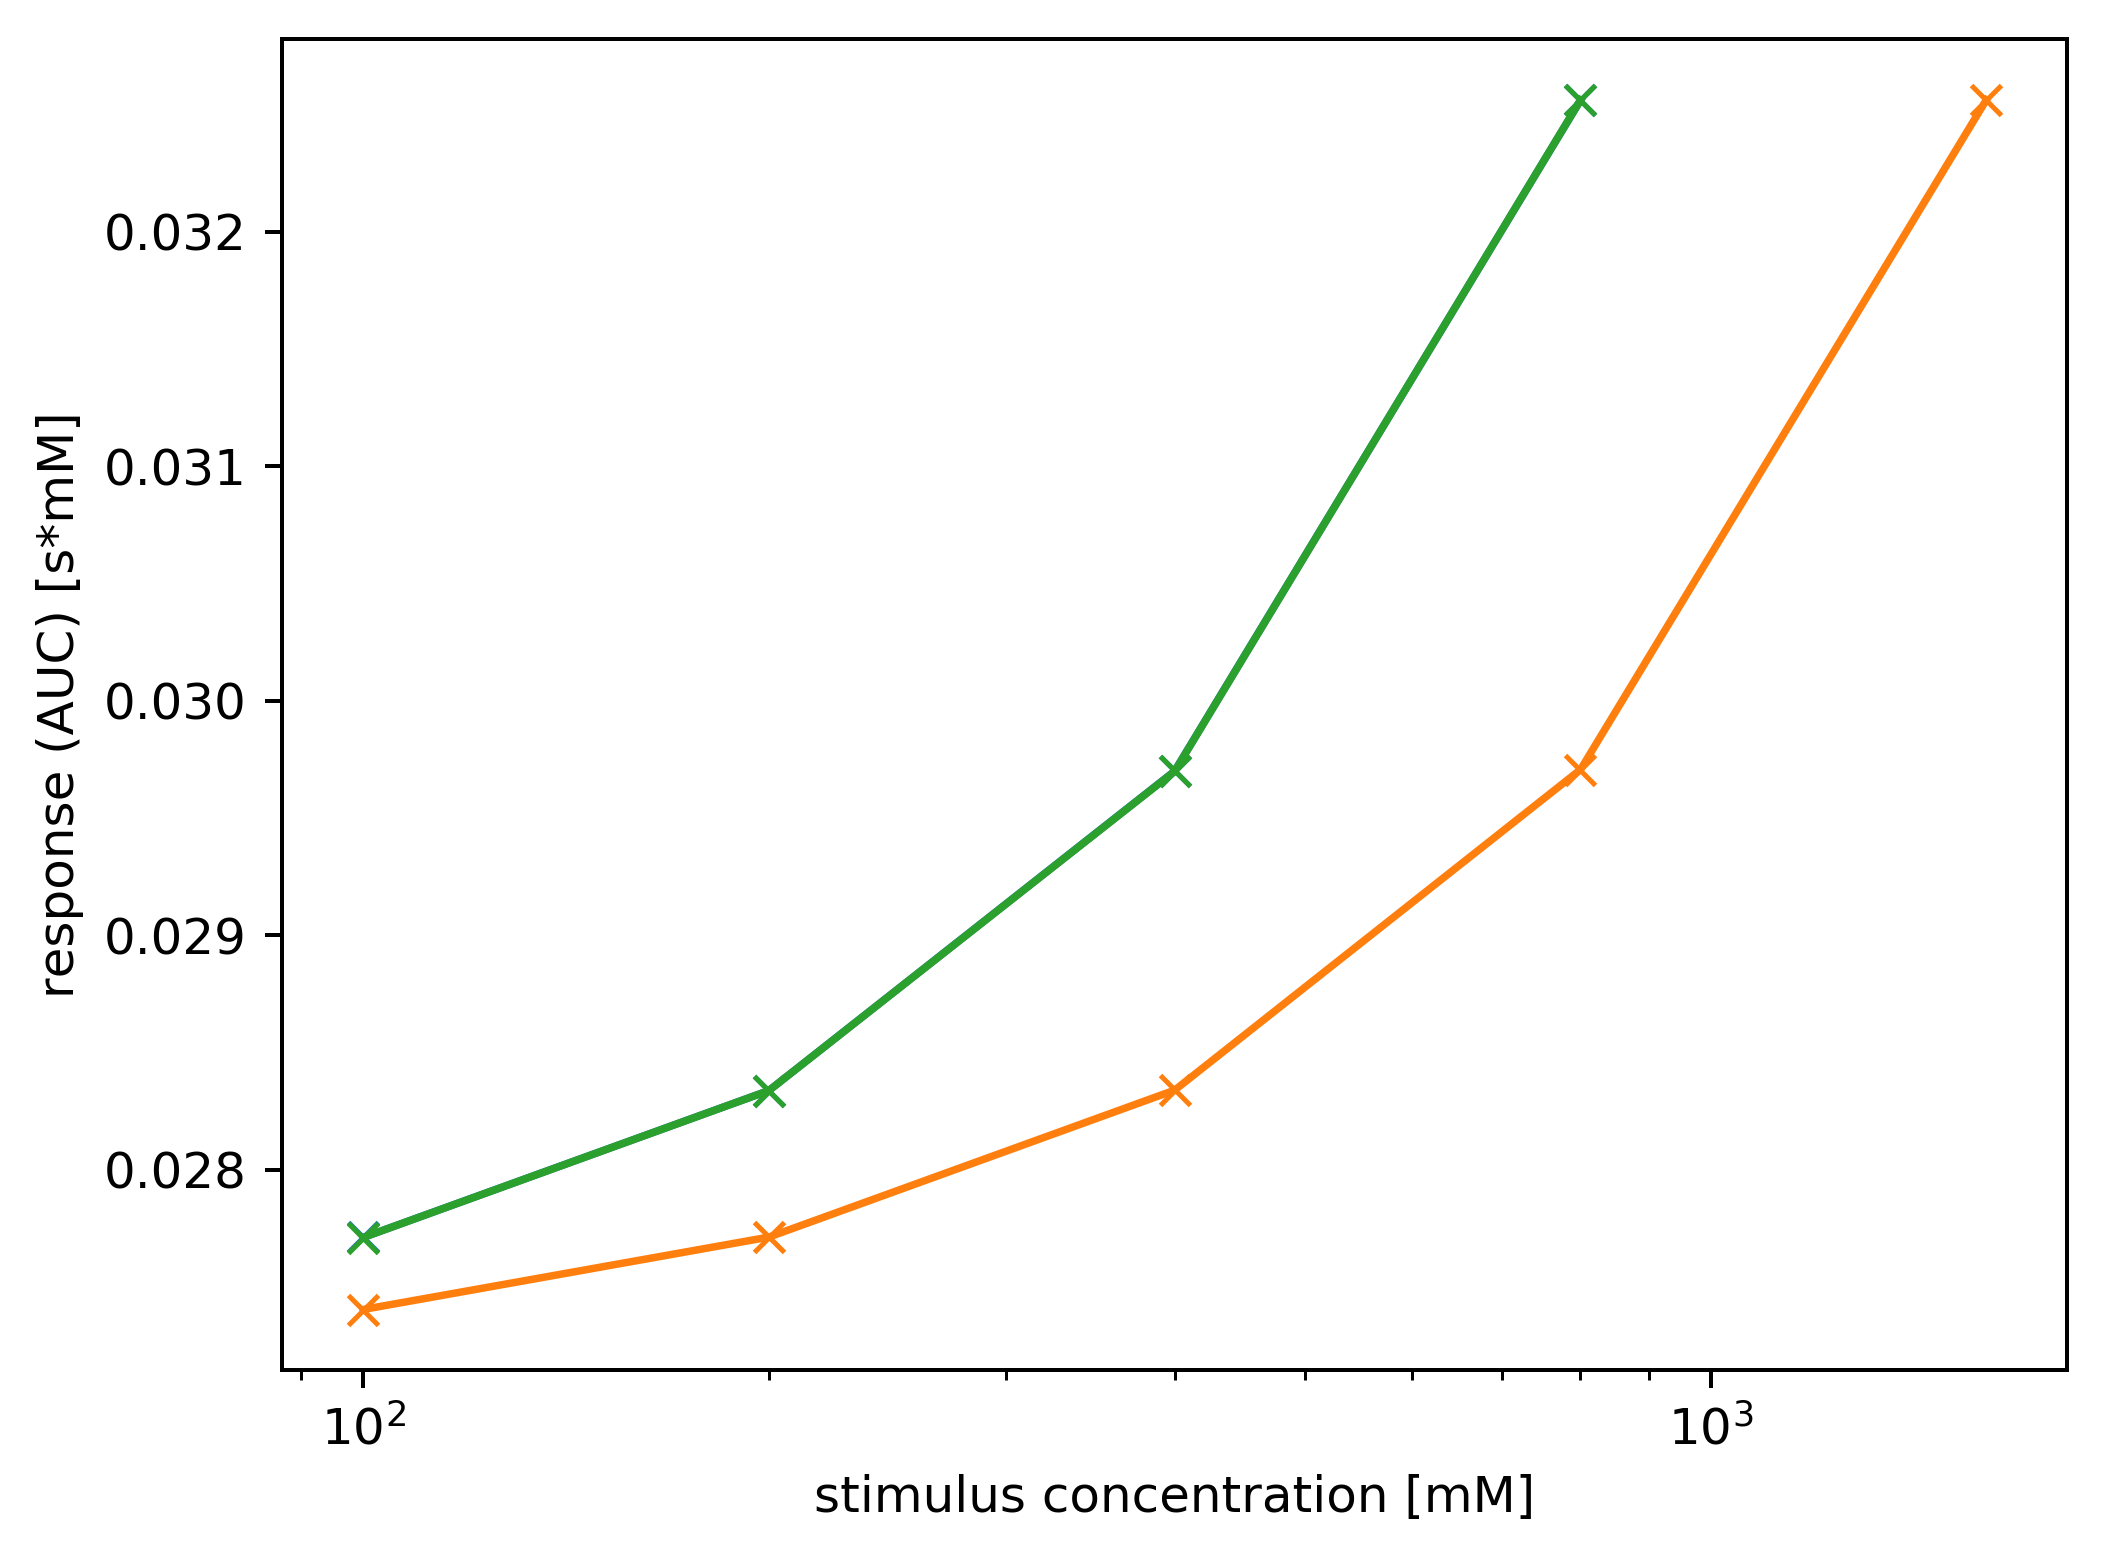
\includegraphics[width=\textwidth]{picture/Drug_response.png}
			\caption{Response of Hog1PPn; initial Glucose at $t=1s$; hyperosmotic shock at $t=30s$} 
			\label{DrugResponseCurve} 
		\end{minipage}
	\end{center}
\end{figure}
It is indicated that a NaCl stimulus results in a higher overall expression of Hog1PPn in contrast to KCl. Furthermore, figure \ref{DrugResponseCurve} visualizes that a sorbitol shock results in even a slight higher overall expression of Hog1PPn per the amount of osmotic active particles.\\ The simulation time was set to 200s, with an initial glucose stimulus at $t=1s$ and the unique hyperosmotic shock at $t=30s$. \\\\
As we can see in figure \ref{SingleDose}, multiple stimulus at predefined times are possible with the model and with the software environment. A second stimulus does not results in the same volume $V$ and turgor pressure $\pi_t$ drop as the first one. Cause of clarity, only a set of ODE are visualized. They represent the other ODEs, because they are the output of multiple interacting components. \newpage
\begin{figure}[h!]
	\begin{center}
		\begin{minipage}{0,85\textwidth}
			
			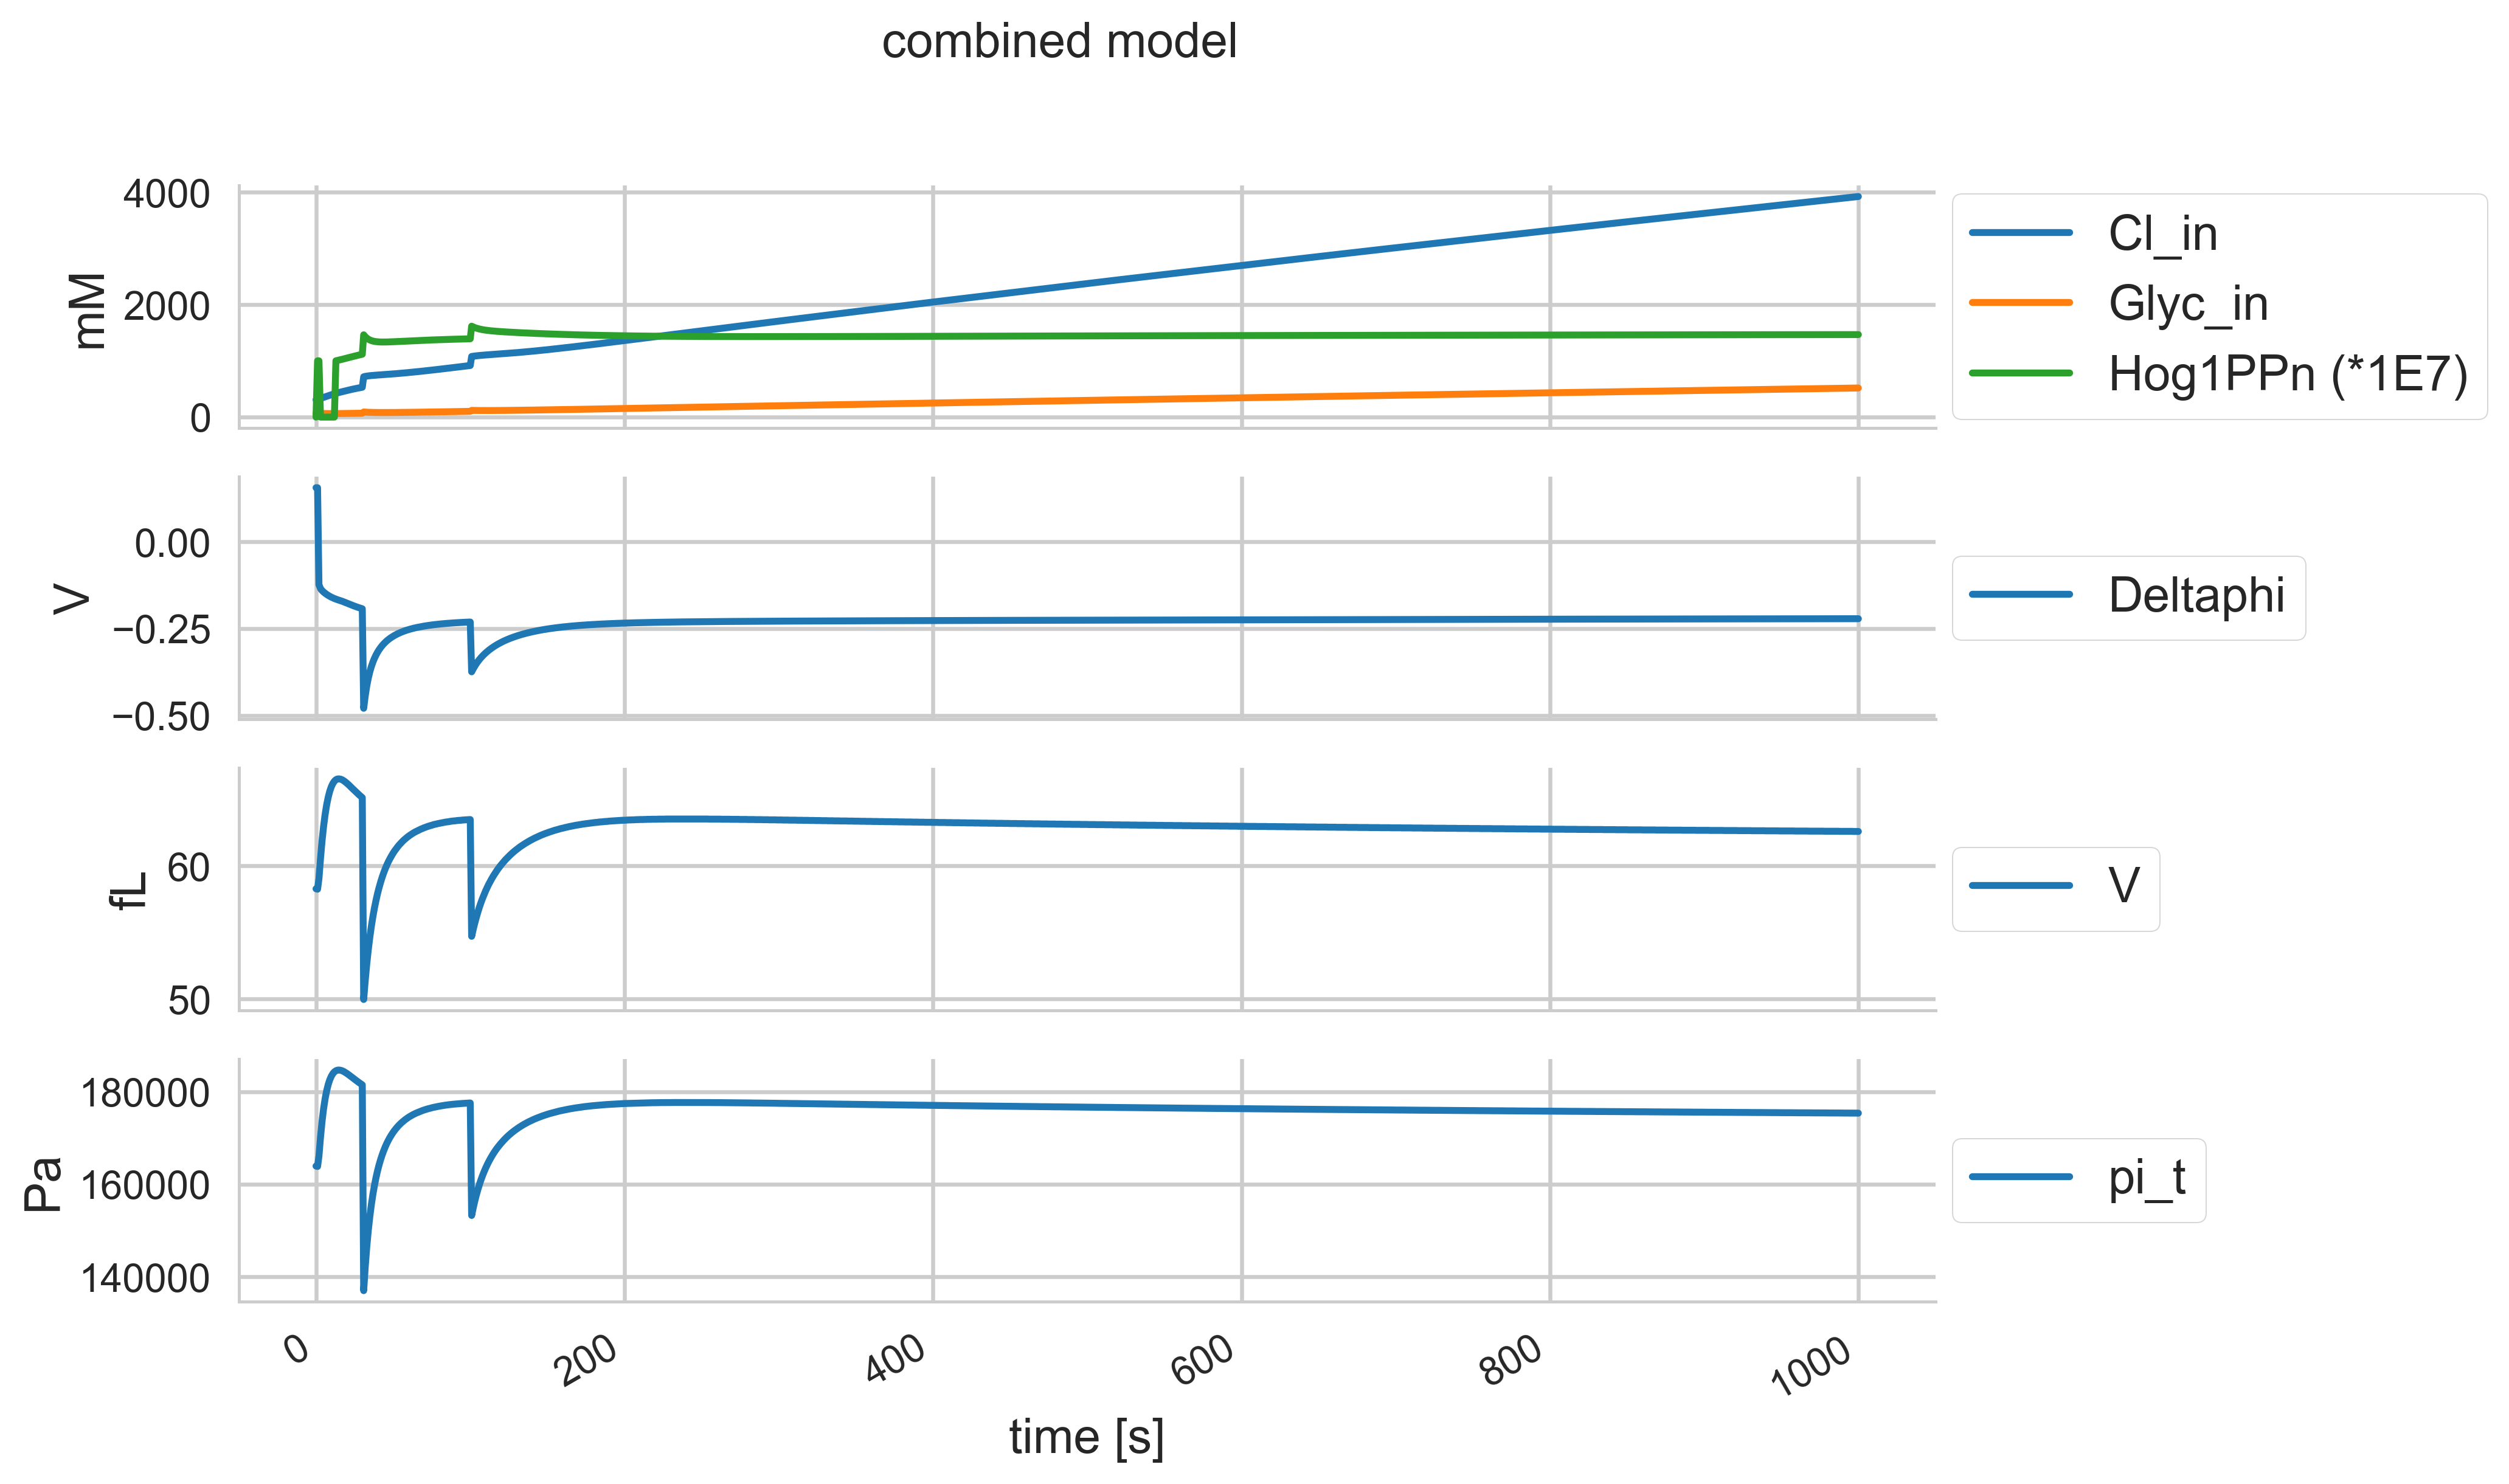
\includegraphics[width=\textwidth]{picture/combined_models_71.png}
			\caption{visualized results of a selected set of ODEs from the combined model} 
			\label{SingleDose} 
		\end{minipage}
	\end{center}
\end{figure}

\subsubsection{Single models with the initial values from the combined model}
We further asked us how each of the original paper model would behave, if they have the initial values of the combined model inherited.\\\\
Every simulation was executed under the condition of a 200 mM NaCl impulse at $t=30s$:\\
\begin{figure}[h!]
	\begin{center}
		\begin{minipage}{0,8\textwidth}
			
			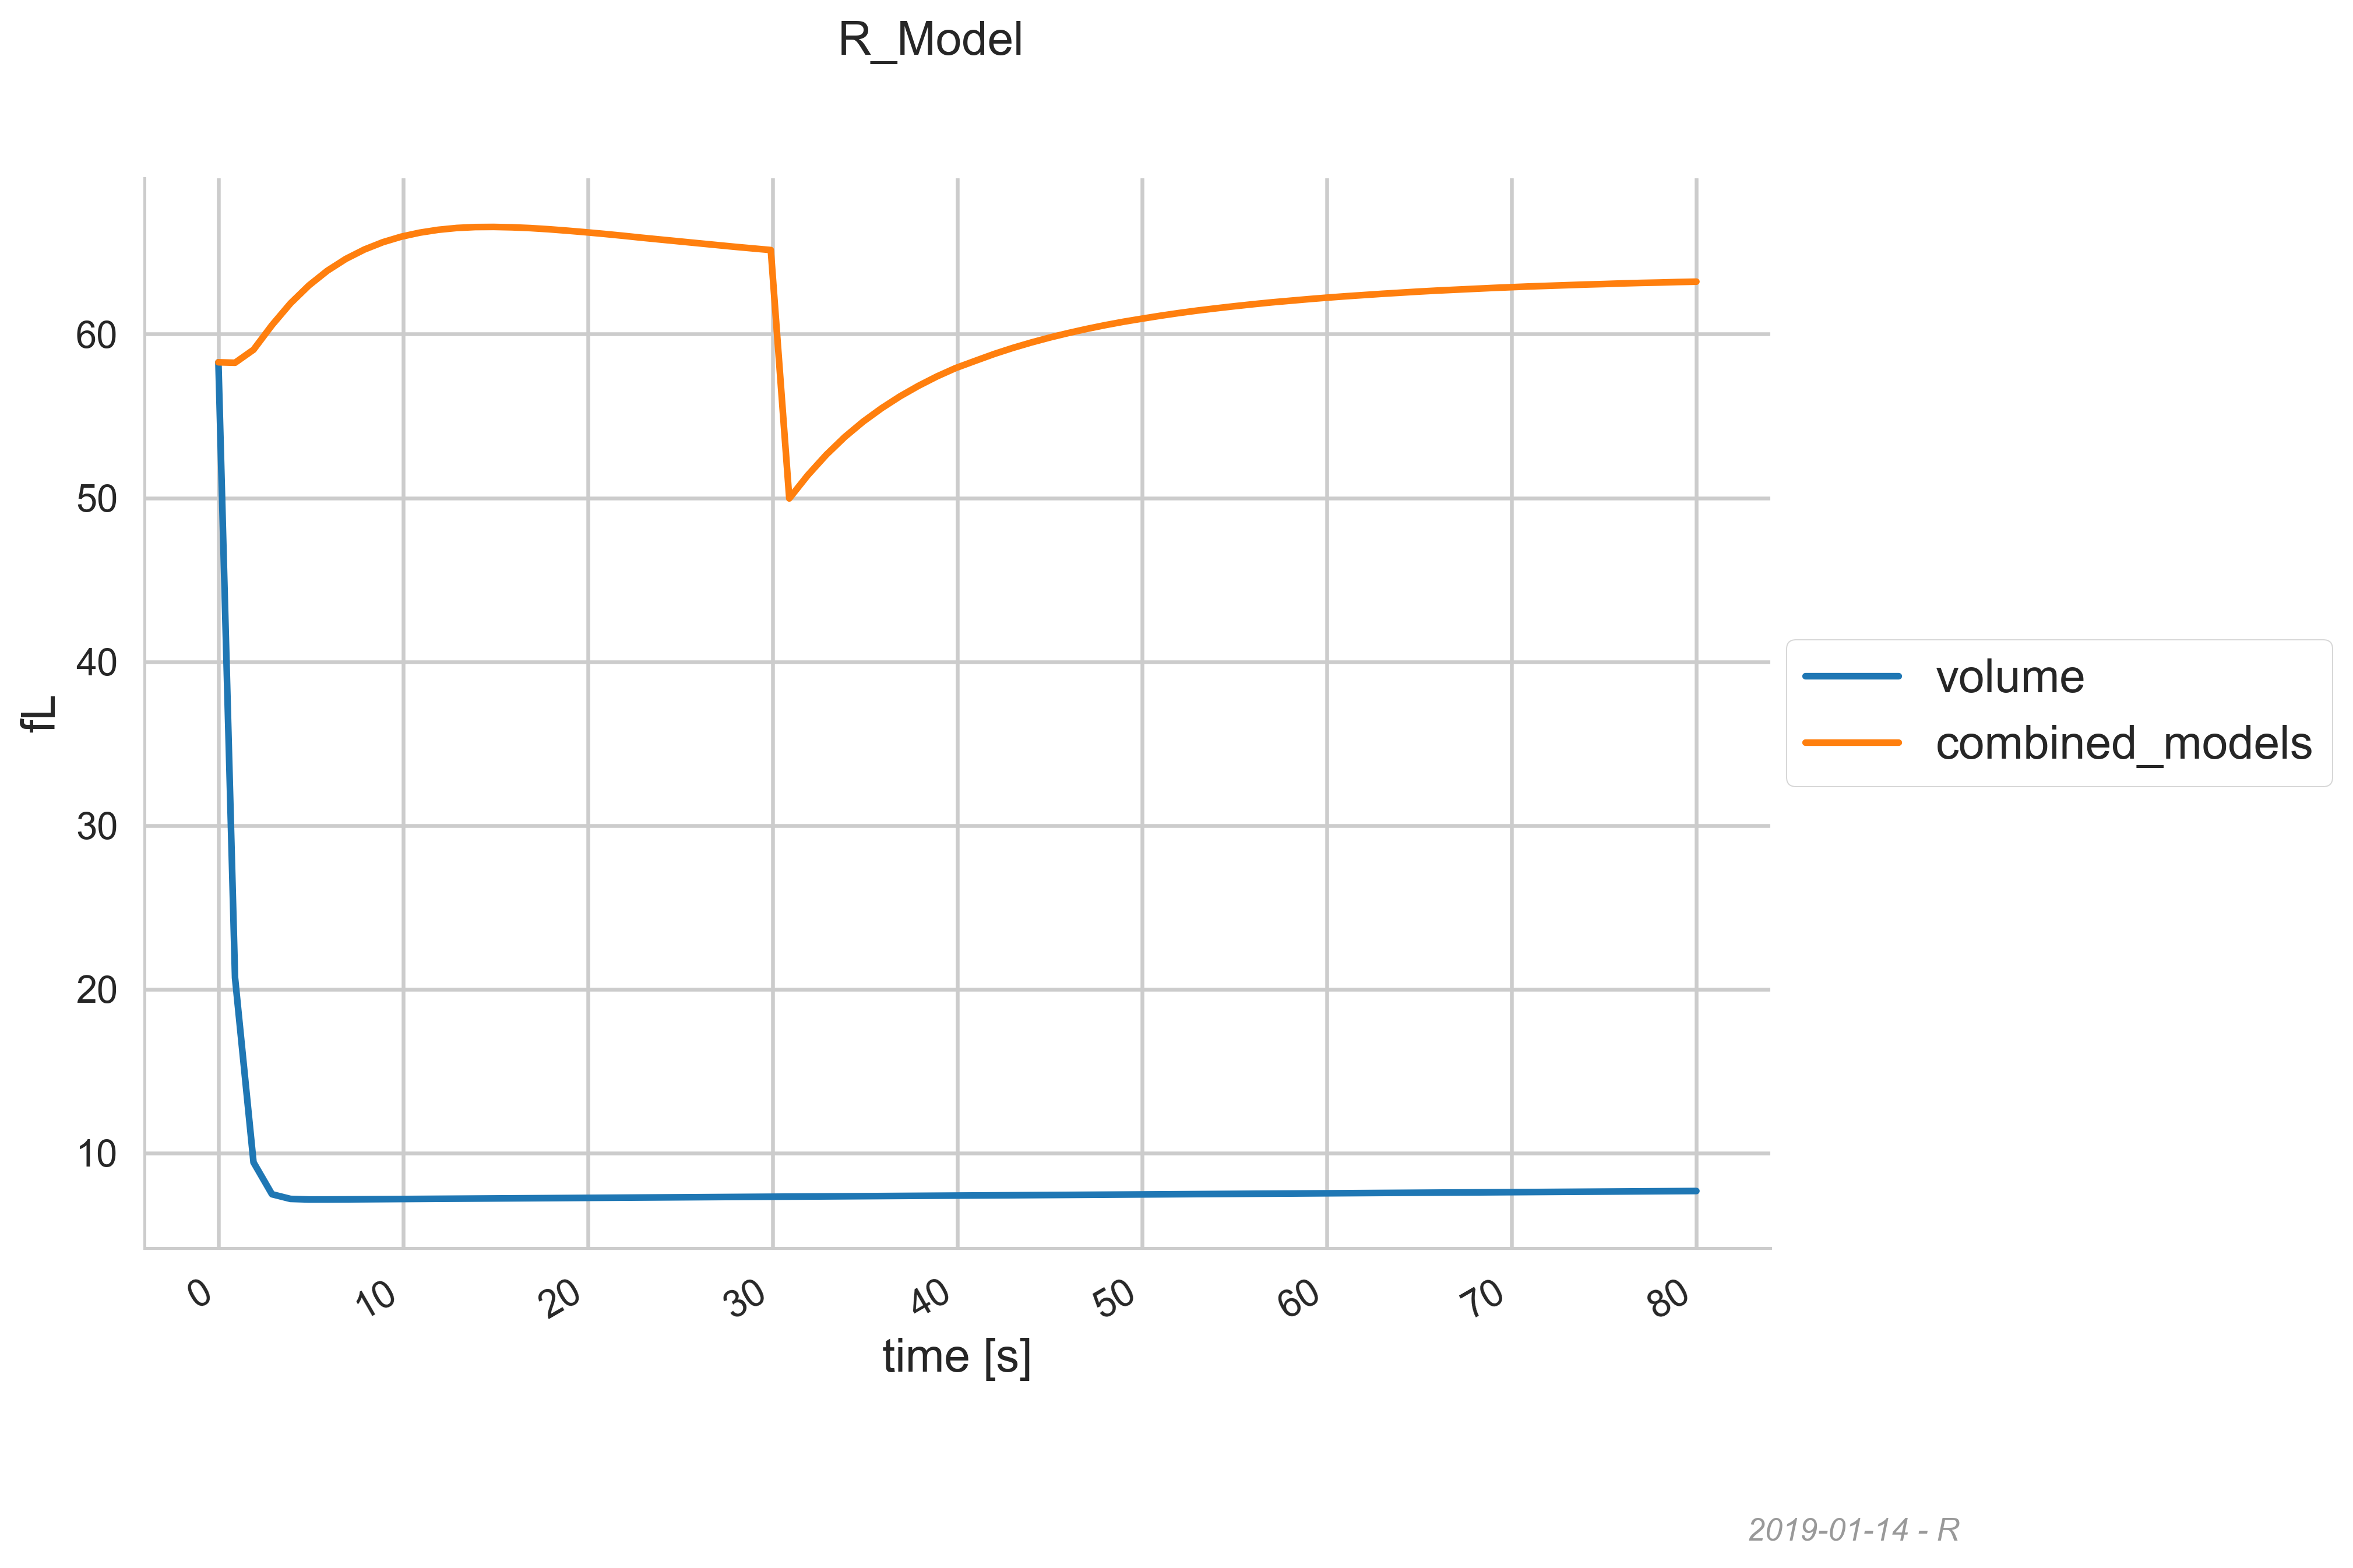
\includegraphics[width=\textwidth]{picture/r_71.png}
			\caption{Responses of the volume $V$} 
			\label{CombiInitVolume} 
		\end{minipage}
	\end{center}
\end{figure}
\begin{figure}[h!]
	\begin{center}
		\begin{minipage}{0,8\textwidth}
			
			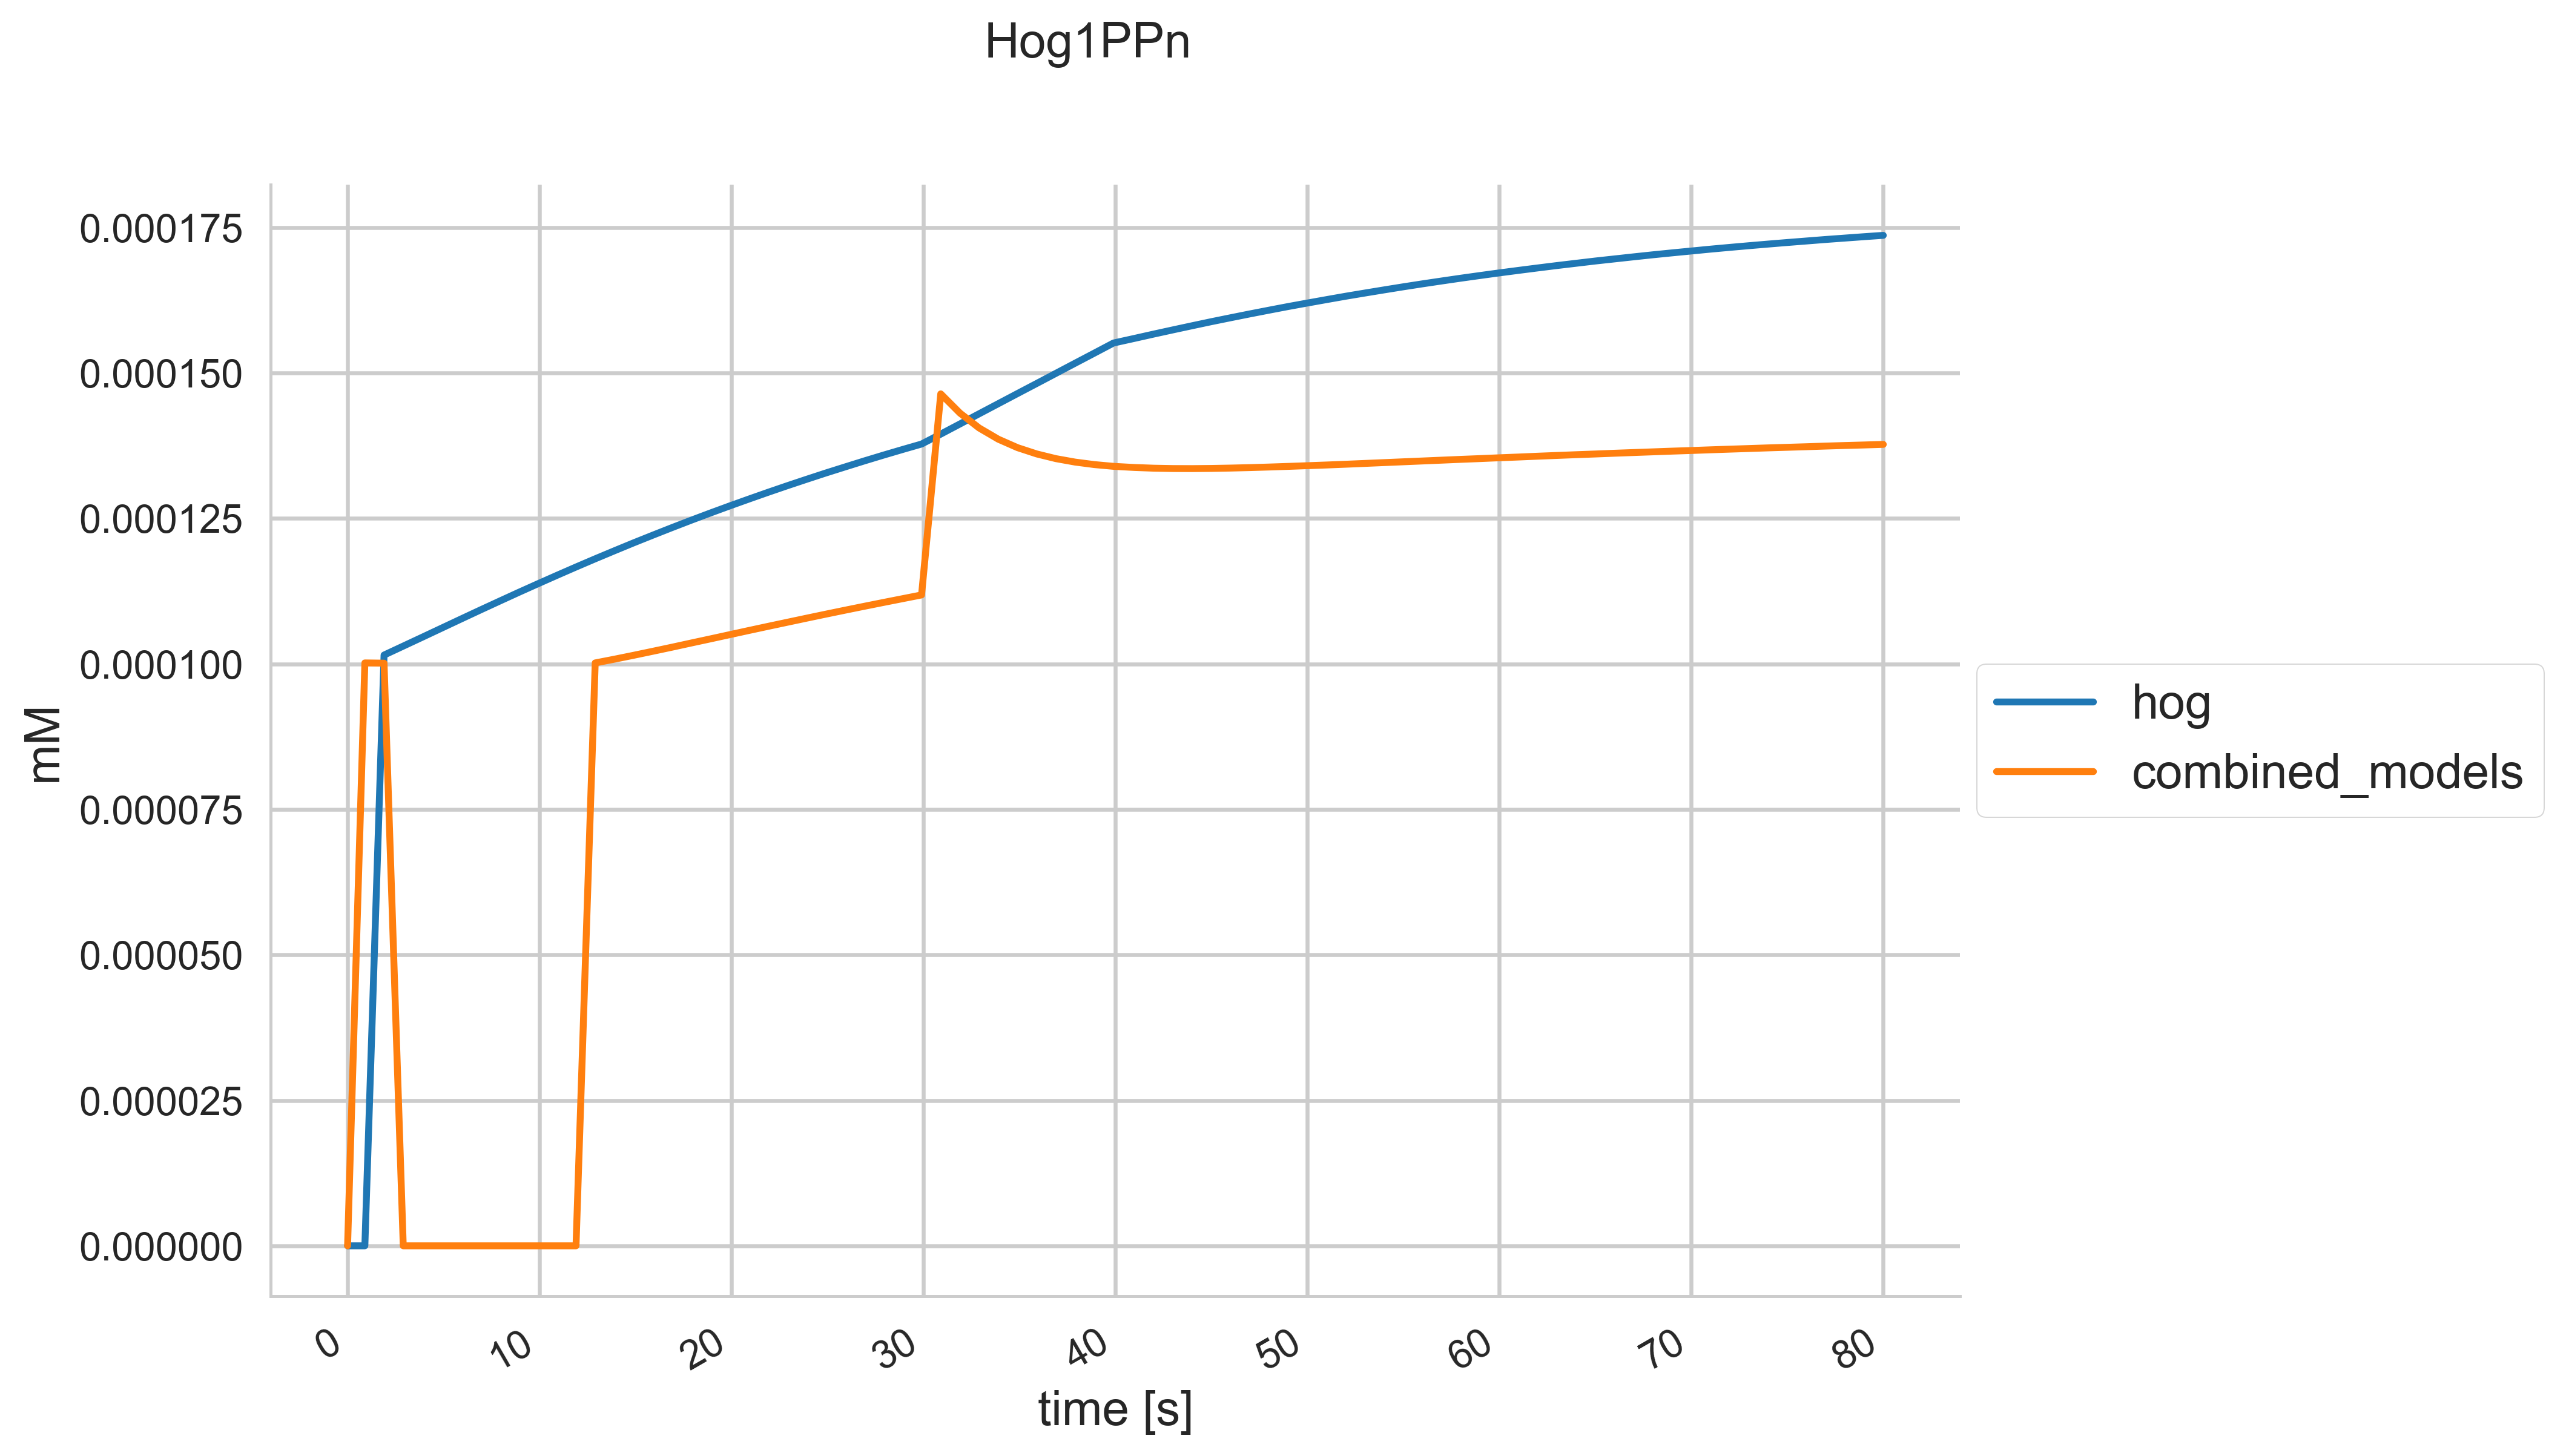
\includegraphics[width=\textwidth]{picture/Hog1PPn_71.png}
			\caption{Response of Hog1PPn; hog model with 200 mM NaCl shock for $t=30-40s$} 
			\label{CombiInitHog} 
		\end{minipage}
	\end{center}
\end{figure}
\begin{figure}[h!]
	\begin{center}
		\begin{minipage}{0,8\textwidth}
			
			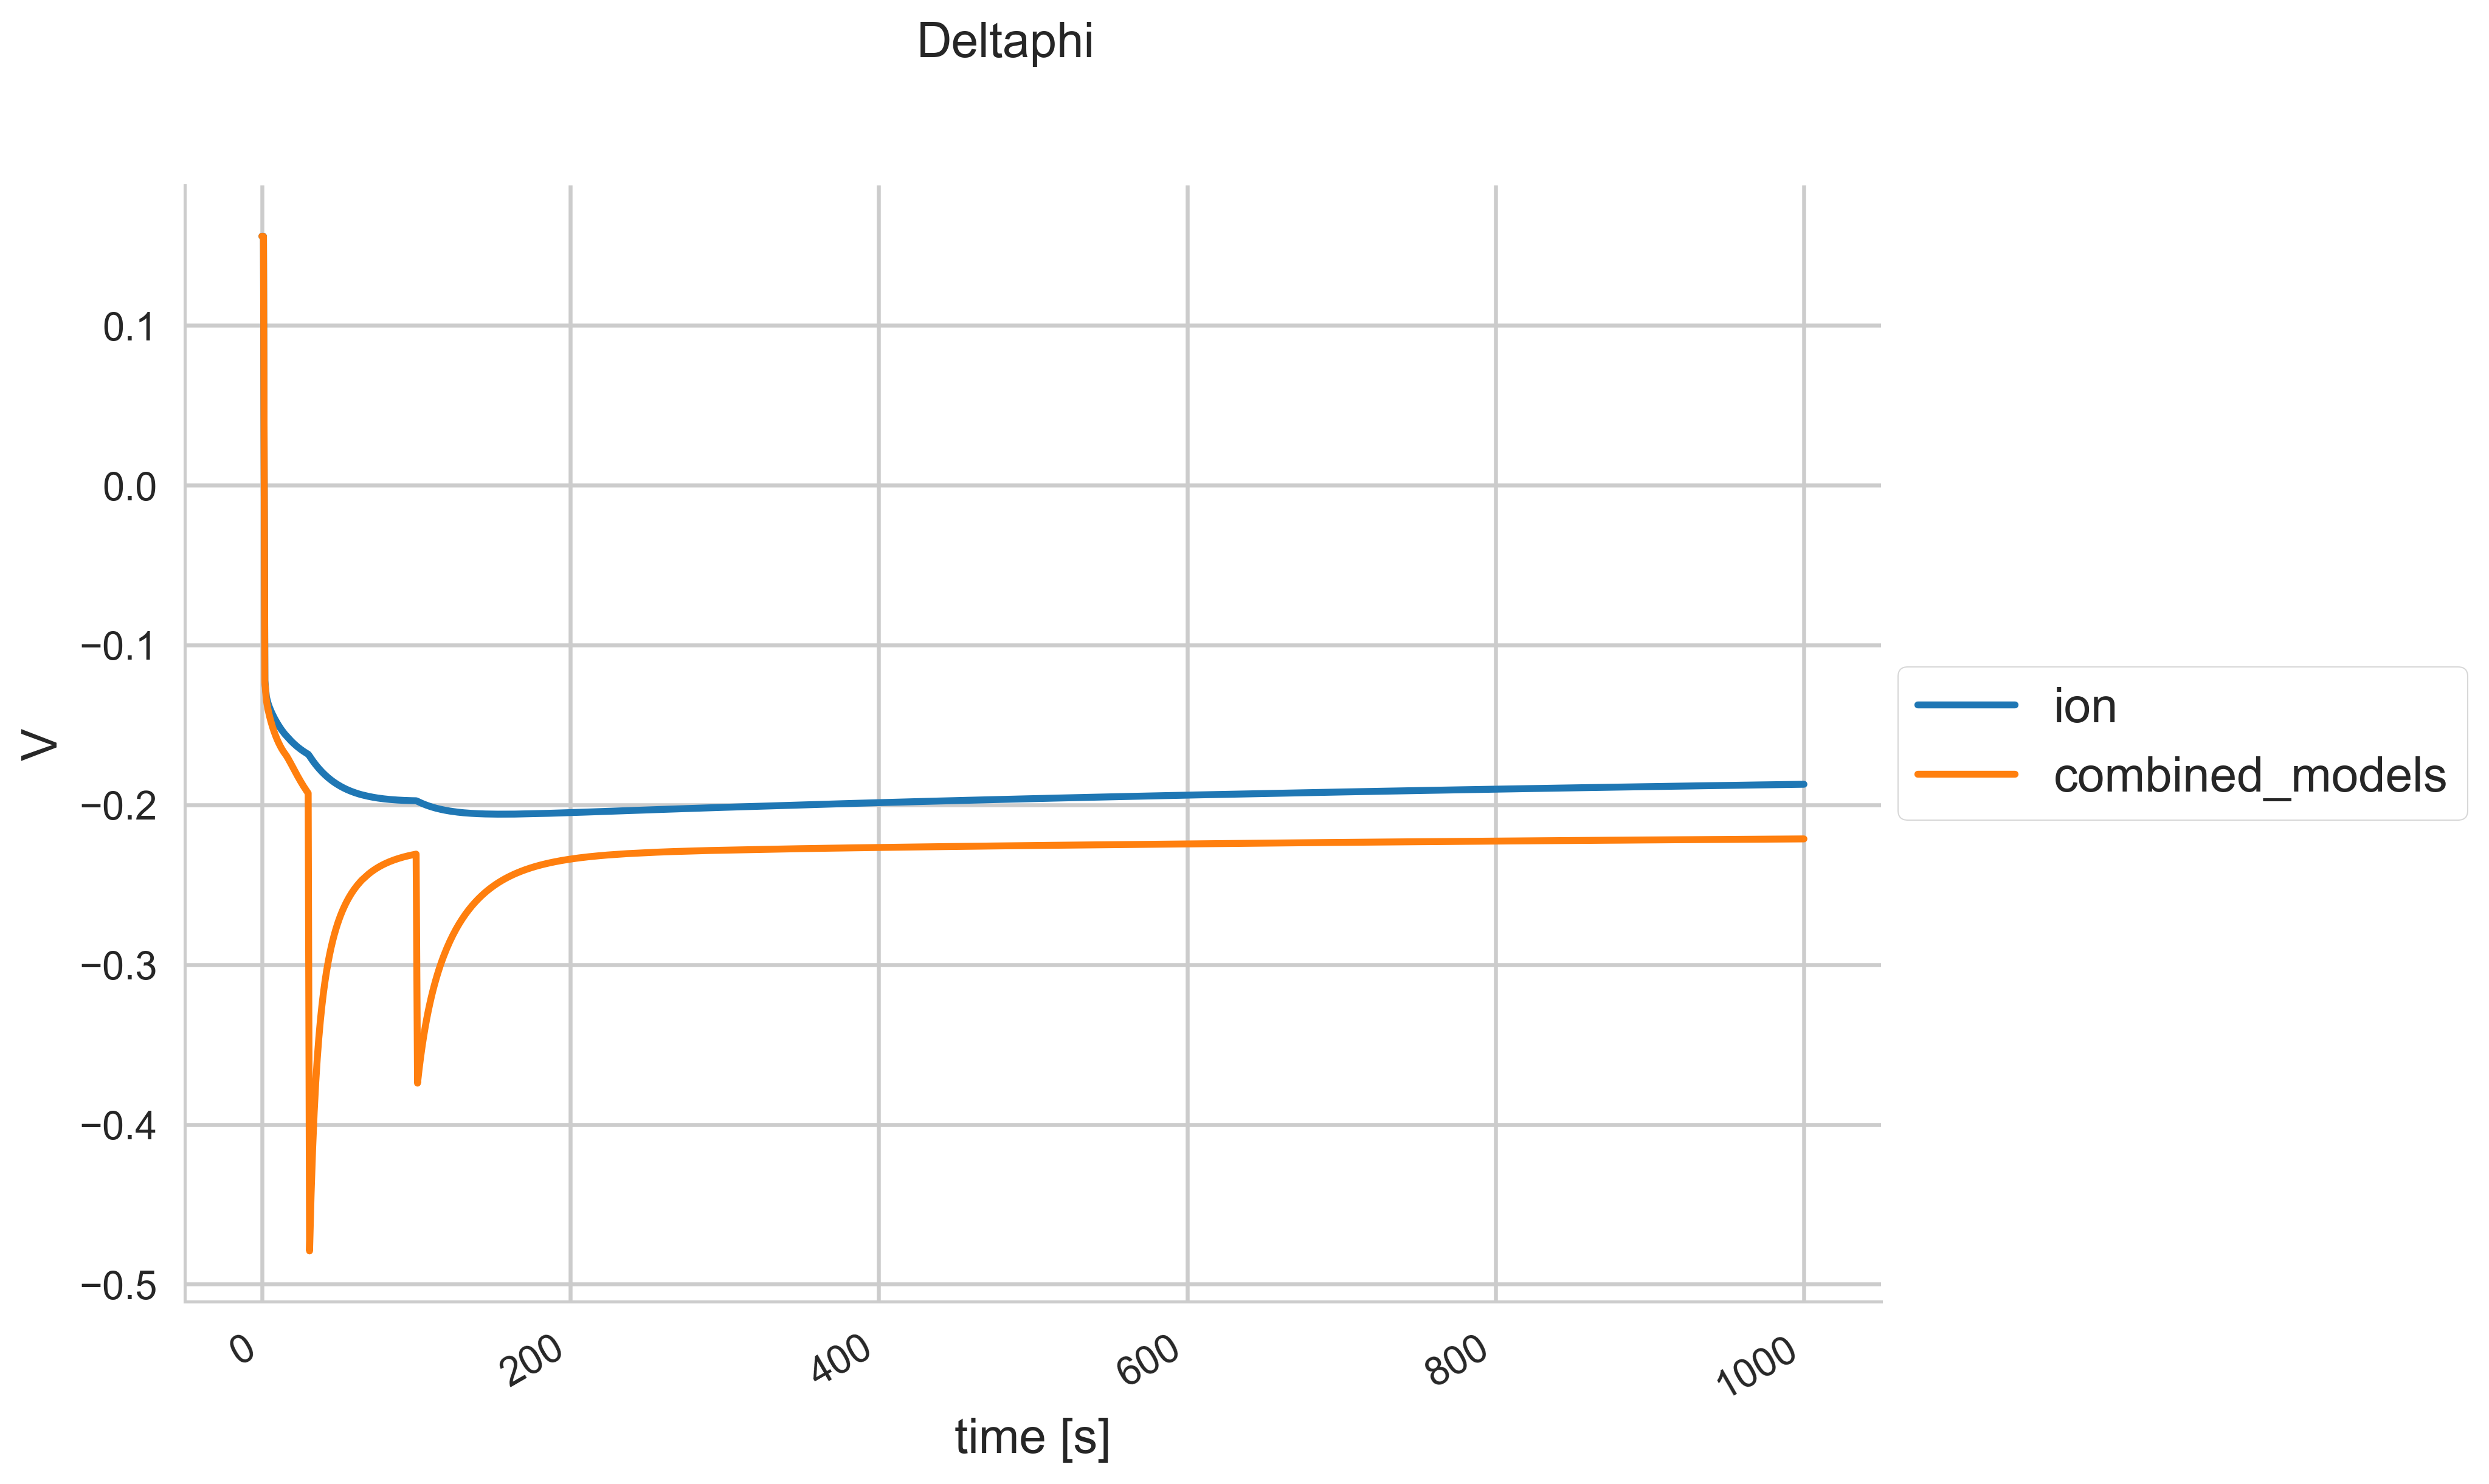
\includegraphics[width=\textwidth]{picture/Deltaphi_71.png}
			\caption{Response of the membrane potential Deltaphi; a second stimulus of 200 mM NaCl at $t=100s$ } 
			\label{CombiInitIon} 
		\end{minipage}
	\end{center}
\end{figure}
Figure \ref{CombiInitVolume} illustrates that the initial values from the combined model for the volume model ODE components does not fit at all. The model ODEs quickly reach a steady state far below from the combined model. It does not exists a drop in volume when faced with a stimulus. The volume model assumes the external osmolyte concentration $c_e$ and corresponding external pressure $\pi_e$ as a constant. It simply does not has an interface for noticing a rise in $c_e$ in a running simulation under the used software development conditions.\\\\
On the other hand, figure \ref{CombiInitHog} and \ref{CombiInitIon} show similarly results between the corresponding models. It is shown in figure \ref{CombiInitIon} that in the combined model the ion fluxes representing membrane potential Deltaphi shows a more dynamically behavior in the interplay with volume and hog pathway regulation. Deltaphi from the ion model drops only slightly. After the adaption to the second stimulus, Deltaphi behaves approximately the same.\\\\\\\\

\newpage
